\documentclass[../main_proj4_correct_template.tex]{subfiles}

\graphicspath{{\subfix{figures/}}}

\begin{document}

\onecolumngrid
\appendix
\section{Appendix A}\label{app:p4_AppendixA}

\subsection{The microstates of the $2\times 2$ ising model}\label{app:p4_AppendixA_microstates}

There are five macrostates for the $2\times 2$ ising model, these are $N\uparrow \in[0, 4]$. By equation \eqref{eq:p4_multiplicty} we also know the number of microstates that are available for each macrostate.

\begin{itemize}
    \item For $N\uparrow=0$ the multiplicity is only 1:
$$
N \uparrow= 0 
\quad \implies \quad
\mathbf{s}_0 = 
\begin{matrix}
    \downarrow & \downarrow \\
    \downarrow & \downarrow 
\end{matrix} \quad,
$$
for which the total energy becomes $E(\mathbf{s}_0)= - 8 J$. 
\item For $N\uparrow=1$ the multiplicity is 4 all of which can be created by shifting the single $s_i=+1$ dipole through the four positions:
$$
N \uparrow= 1 
\quad \implies \quad
\mathbf{s}_1 = 
\begin{matrix}
    \uparrow & \downarrow \\
    \downarrow & \downarrow 
\end{matrix} \quad,
$$
the total energy becomes $E(\mathbf{s}_1)= 0 J$. 
\item For $N\uparrow=2$ the multiplicity is 6. There are three structures which is needed to cover all posibilities:
$$
N \uparrow= 2
\implies
\mathbf{s}_{2a} = 
\begin{matrix}
    \uparrow & \downarrow \\
    \uparrow & \downarrow 
\end{matrix}, \mathbf{s}_{2b} = 
\begin{matrix}
    \uparrow & \uparrow \\
    \downarrow & \downarrow 
\end{matrix}, \mathbf{s}_{2c} = 
\begin{matrix}
    \uparrow & \downarrow \\
    \downarrow & \uparrow 
\end{matrix},
$$
for which the total energy becomes $E(\mathbf{s}_{2a})= E(\mathbf{s}_{2b})=0 J$ and $E(\mathbf{s}_{2c}) = 8J$.
\item For $N\uparrow=3$ the story is analog to that of $N\uparrow=1$ and for $N\uparrow=4$ it's analog to that of $N\uparrow=0$.
\end{itemize}

This yields in total $1+4+6+4+1 = 16 =2^{4}$ microstates.


\subsection{Deriving the analytical expressions for $2 \times 2$ ising model}\label{app:p4_AppendixA_analyticalexpressions}

This appendix shows the derivation of the analytical expression for the partition function and statistical modes for the $2\times 2$ ising model. Specific values are summarized in table \ref{tab:p4_2x2lattice}. 

\subsubsection{The partition function - $Z$}\label{app:p4a_partition_function}

The general expression for the partition function is given by equation \eqref{eq:p4_partition_function}. Since we are taking the sum we can use the degeneracy of the energy to weight the exponential functions:

\begin{equation*}
\begin{split}
Z & = \sum\limits_{\mathbf{s}^{(j)} \in \mathcal{S}} e ^{ - \beta E(\mathbf{s}^{(j)})} \\
&= e ^{ - \beta E(\mathbf{s}_0)} + 4e ^{ - \beta E(\mathbf{s_1})} + 4e ^{ - \beta E(\mathbf{s}_{2a})} \\
&\quad +2 e ^{ - \beta E(\mathbf{s}_{2b})} + 4e ^{ - \beta E(\mathbf{s}_3) } + e ^{ - \beta E(\mathbf{s}_4)} 
\end{split}
\end{equation*}

\noindent where we have used the subscript of $\mathbf{s}$ to denote which of the macrostates the vector describes (see Appendix \ref{app:p4_AppendixA_microstates} for descriptions of macrostates). Since $E(\mathbf{s}_0) = E(\mathbf{s}_4) = -8 J$ and $E(\mathbf{s}_1) = E(\mathbf{s}_{2a}) = E(\mathbf{s}_{3}) = 0 J$ we get

\begin{equation*}
Z = 2e^{8 J\beta } + 12 + 2e^{-8 J\beta } \quad.
\end{equation*}

\noindent Here we can use the definition of $\cosh(x) = \frac{e^x+e^{-x}}{2}$ and the change of variables $x=8J\beta$ to recognize that 

$$2e^{x} + 2e^{-x} = 4\frac{e^x+e^{-x}}{2} \implies 4 \cosh(8J\beta) \quad, $$

\noindent and so the final expression for the partition function becomes;

\begin{equation*}
    Z = 12 + 4\cosh(8J\beta) \quad.
\end{equation*}

\subsubsection{The expectation value of the energy per spin - $\langle\epsilon \rangle$}\label{app:p4a_expectation_energyperspin}

To analytically derive an expectation value for $\epsilon$ which a function of the random variable (microstate) $\mathbf{s}$ we use
\begin{equation*}
    \mathbb{E}[\epsilon] 
    = \langle \epsilon \rangle 
    = \frac{1}{N}\langle E\rangle 
    = \frac{1}{N} \sum\limits_{\mathbf{s}^{(j)} \in \mathcal{S}} E(\mathbf{s}^{(j)}) p(\mathbf{s}^{(j)}) \quad ,
\end{equation*}

\noindent where $p(\mathbf{s}^{(j)})$ is the probability of observing the system in the microstate $j$. By writing out $p(\mathbf{s}^{(j)})$ in accordance with equation \eqref{eq:p4_Boltzmann_distribution} we get

\begin{equation*}
    \mathbb{E}[\epsilon] 
    = \frac{1}{NZ}\sum\limits_{\mathbf{s}^{(j)}} E(\mathbf{s}^{(j)}) e^{-\beta E(\mathbf{s}^{(j)})} \quad. 
\end{equation*}

\noindent The partial derivative of $e^{-\beta E(\mathbf{s}^{(j)}}$ with respect to $\beta$ is $-E(\mathbf{s}^{(j)}) e^{-\beta E(\mathbf{s}^{(j)}}$ and so the expression is simplified to 
\begin{equation*}
    -\frac{1}{NZ} \frac{\partial}{\partial\beta} \sum\limits_{\mathbf{s}^{(j)}} e^{-\beta E(\mathbf{s}^{(j)}} \quad, 
\end{equation*}

\noindent where the partial derivative has been taken out of the sum because of the sum rule of derivatives. The summation in this expression now simply accounts to the partition function of equation \eqref{eq:p4_partition_function}. Using the specific partition function of the two dimensional $2\times 2$ Ising model the derivative becomes 

\begin{equation*}
\begin{split}
    \frac{\partial Z}{\partial\beta} &= \frac{\partial }{\partial\beta}\bigg[ 12 + 4cosh(8J\beta)\bigg] \\
    &= 4\frac{\partial }{\partial\beta}\bigg[ 8J\beta\bigg] \frac{\partial }{\partial u}\bigg[cosh(u)\bigg] \\
    &=32 J sinh(8J\beta) \quad,
    \end{split}
\end{equation*}

\noindent which yields the final expression 

\begin{equation*}
    \mathbb{E}[\epsilon] = - \frac{1}{N}\frac{32Jsinh(8J\beta)}{Z} \quad.
\end{equation*}

Similary we can derive the expectation value for the squared $\epsilon$ by:

\begin{equation*}
\begin{split}
    \mathbb{E}[\epsilon^{2}] & = \frac{1}{N^{2}} \langle E^{2}\rangle \\
    &= \frac{1}{N^{2}} \sum\limits_{\mathbf{s}^{(j)} \in \mathcal{S}} E^{2}(\mathbf{s}^{(j)}) p(\mathbf{s}^{(j)}) \\
    &= \frac{1}{N^{2}Z} \sum\limits_{\mathbf{s}^{(j)} \in \mathcal{S}} E^{2}(\mathbf{s}^{(j)}) e^{-\beta E(\mathbf{s}^{(j)})} \\
\end{split}    
\end{equation*}

\noindent where the summed-over portion is equal to the second order derivative of the exponential part $\frac{\partial^{2}}{\partial \beta^{2}}\big[e^{-\beta E(\mathbf{s}^{(j)})}\big] = E^{2}(\mathbf{s}^{(j)}) e^{-\beta E(\mathbf{s}^{(j)})}$. Using this we can write the expectation value as

\begin{equation*}
    \mathbb{E}[\epsilon^{2}] = \frac{1}{N^{2}Z} \frac{\partial^{2}Z}{\partial \beta^{2}} \quad,
\end{equation*}

\noindent which for this specific means we solve

\begin{equation*}
\begin{split}
    \frac{\partial^{2}Z}{\partial \beta^{2}} &= \frac{\partial^{2}}{\partial \beta^{2}} \bigg[ 12 + 4cosh(8J\beta)\bigg] \\
    &= \frac{\partial}{\partial\beta}\bigg[32 J sinh(8J\beta)\bigg] \\
    &=256 J^{2} cosh(8J\beta) \quad.
\end{split}
\end{equation*}

\noindent The full expectation value is therefor;

\begin{equation*}
    \mathbb{E}[\epsilon^{2}] = \frac{1}{N^{2}}\frac{256 J^{2} cosh(8J\beta)}{Z} \quad.
\end{equation*}



\subsubsection{The expectation value of the magnetization per dipole - $\langle |m|\rangle$}

To analytically derive an expectation value for the absolute value of the magnetization per dipole we start with 

\begin{equation*}
    \mathbb{E}[|m|] = \frac{1}{N} \langle|M|\rangle = \frac{1}{N} \sum\limits_{\mathbf{s}^{(j)} \in \mathcal{S}} |M(\mathbf{s}^{(j)})| P(\mathbf{s}^{(j)}) \quad.
\end{equation*}

\noindent From table \ref{tab:p4_2x2lattice} we know that the magnetization only takes on three absolute values: $2\operatorname{microstates with }|M|=4$ (with $2*E=-8J$), $8\operatorname{microstates with }|M|=2$ (with $8*E=0J$ which implies that the Boltzmann factor is 1) and lastly $6\operatorname{microstates with }|M|=0$ so the contribution will be zero for these microstates. Writing out the sum this yields

\begin{equation*}
\begin{split}
    \mathbb{E}[|m|] &= \frac{1}{NZ}\bigg( 2(4 e^{-\beta(-8)J}) +8(2\cdot1) + 6\cdot 0\bigg) \\
    &= \frac{8}{N} \frac{2+e^{\beta 8 J}}{Z} \quad,
\end{split}   
\end{equation*}

\noindent for which the latter is the final analytical expression. Similarly we can derive the expression for the squared magnetization per dipole as; 

\begin{equation*}
\begin{split}
    \mathbb{E}[m^{2}] & = \frac{1}{N^{2}} \mathbb{E[M^{2}]} \\
    &= \frac{1}{N^{2}Z} \sum\limits_{\mathbf{s}^{(j)} \in \mathcal{S}} M^{2}(\mathbf{s}^{(j)})e^{-\beta E(\mathbf{s}^{(j)})} \\
    &= \frac{1}{N^{2}Z} \bigg( 2(4^{2} e^{-\beta(-8)J}) +8(2^{2}\cdot1) + 6\cdot 0\bigg) \\
    &= \frac{32}{N^{2}} \frac{1+ e^{\beta 8J}}{Z} \quad.
\end{split}
\end{equation*}

\subsubsection{The heat capacity per dipole - $C_V/N$}\label{app:p4a_Cv}

The heat capacity normalized per dipole can be expressed by 
\begin{equation*}
    \frac{C_V(T)}{N} = \frac{N}{k_BT^{2}} \operatorname{Var}(\epsilon) \quad, 
\end{equation*}

\noindent where the variance is 

\begin{equation*}
\begin{split}
    \operatorname{Var}(\epsilon) &= \Big[ \mathbb{E}[\epsilon^{2}] - (\mathbb{E}[\epsilon])^{2}\Big] \\
    &= \left(\frac{1}{N^{2}}\frac{256 J^{2} cosh(8J\beta)}{Z}\right)- \left(- \frac{1}{N}\frac{32Jsinh(8J\beta)}{Z}\right)^{2} \\
    &= \frac{256J^{2}}{N^{2}Z} \left( cosh(8J\beta) - \frac{4}{Z}sinh^{2}(8J\beta) \right) \quad. 
\end{split}
\end{equation*}

\noindent The full analytical expression becomes 

\begin{equation*}
    \frac{C_V(T)}{N} = \frac{256J^{2}}{Nk_BT^{2} Z} \bigg( cosh(8J\beta) - \frac{4}{Z}sinh^{2}(8J\beta) \bigg) \quad.
\end{equation*}

\subsubsection{The magnetic suceptibility per dipole - $\chi/N$}\label{app:p4a_chi}

The  magnetic suceptibility normalized per dipole can be expressed by 
\begin{equation*}
    \frac{\chi(T)}{N} = \frac{N}{k_BT} \operatorname{Var}(m) \quad, 
\end{equation*}

\noindent where the variance is 

\begin{equation*}
\begin{split}
    \operatorname{Var}(m) &= \Big[ \mathbb{E}[m^{2}] - (\mathbb{E}[|m|])^{2}\Big] \\
    &= \bigg(\frac{32}{N^{2}} \frac{1 +e^{\beta8J}}{Z}\bigg) - \bigg(\frac{8}{N}\frac{2+e^{\beta8J}}{Z}\bigg)^{2} \\
    &= \frac{32}{N^{2}Z} \bigg((1+e^{\beta8J}) - \frac{2}{Z}(2+e^{\beta8J})^{2}\bigg)\quad. 
\end{split}
\end{equation*}

\noindent The full analytical expression becomes 

\begin{equation*}
    \frac{C_V(T)}{N} = \frac{32}{Nk_BTZ} \bigg((1+e^{\beta8J}) - \frac{2}{Z}(2+e^{\beta8J})^{2}\bigg) \quad.
\end{equation*}

\newpage
\section{Additional Figures}

\subsection{Convergence of numerical values in $2\times 2$ Ising model}

Figure \ref{fig:p4_appB_p4_convergence} show the numerical estimates for $\mathbb{E}[\epsilon]$, $C_V/N$, $\mathbb{E}[|m|]$, $\chi/N$ at $T = 1~J/k_B$. The numerical values does not, in general, converge until $\sim 10^{4}$ monte carlo cycles. 

\begin{figure}[h!]
    \centering
    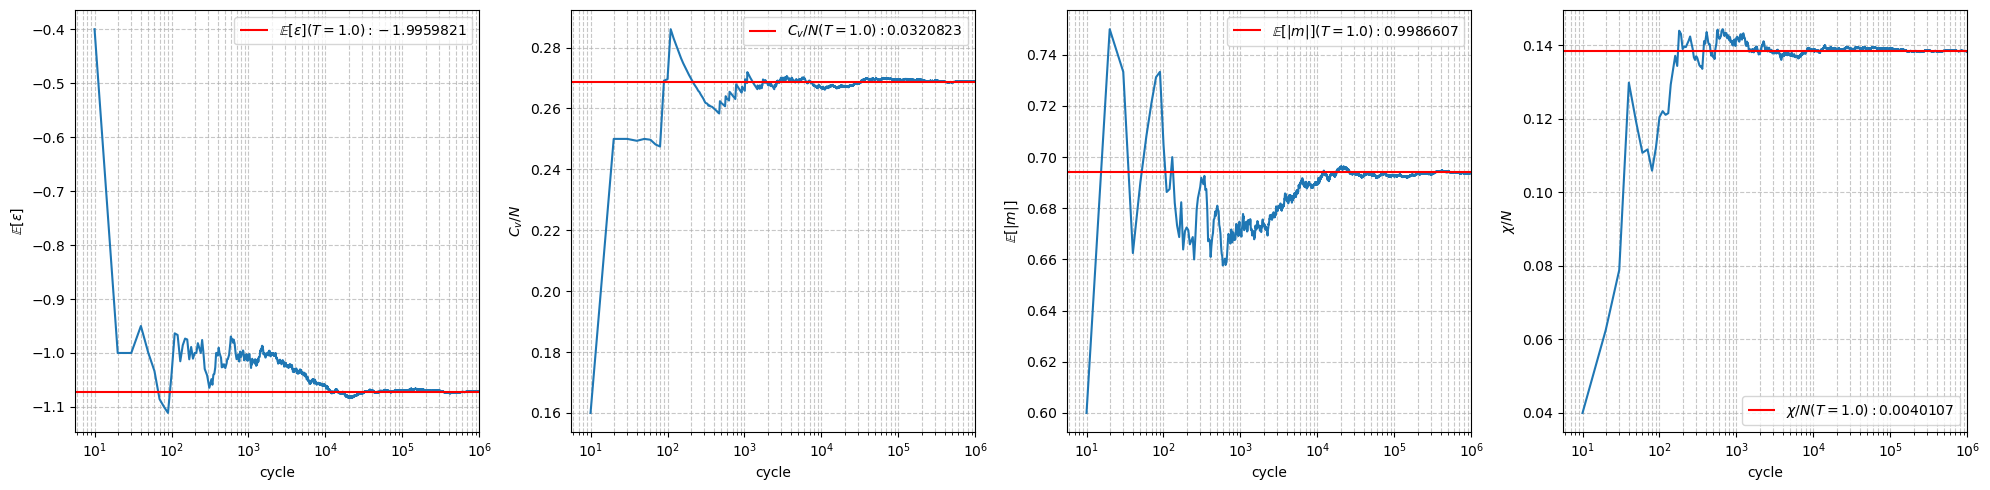
\includegraphics[width=0.8\linewidth]{Project 4/figures/p4_convergence.png}
    \caption{The convergence of numerical estimates towards the analytical values for the $2\times 2$ Ising model. These are values for $T=1~J/k_B$. The blue line shows the numerical estimates, while the red line shows the analytical value.}
    \label{fig:p4_appB_p4_convergence}
\end{figure}

\subsection{Convergence of expectation values in a $20\times 20$ Ising model}

Figure \ref{fig:p4_appb_p5_expectation_convergence} show the convergence of numerically estimated expectation values for $\epsilon$ and $|m|$ in a $20\times 20$ Ising model. It shows how higher temperature increases the energy, but also that the magnitude of magnetization is substantially decreased when surpassing the Curie temperature. 

\begin{figure}[h!]
    \centering
    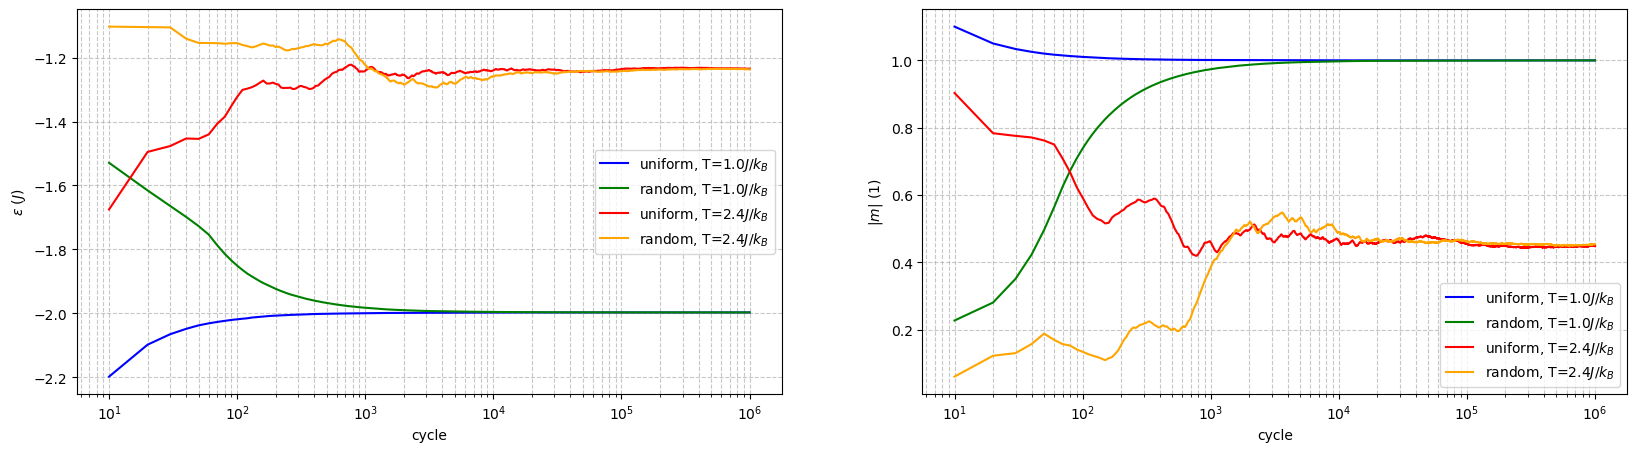
\includegraphics[width=0.8\linewidth]{Project 4/figures/p5_equilibration_expectation.png}
    \caption{The convergence of expectation values estimates for the $20\times 20$ Ising model.}
    \label{fig:p4_appb_p5_expectation_convergence}
\end{figure}

\end{document}


